\chapter{University Ontology}

L'university ontology si occupa di creare un'ontologia riguardante il mondo delle università e gli elementi che le compongono. Con essa è possibile modellare diverse conoscenze come i corsi di laurea presenti, le lezioni dei suoi corsi, i campus, ecc.
In tale relazione vengono presentate le classi e proprietà presenti al fine anche di un possibile riutilizzo in caso si volesse estendere ed usare su larga scala.

\section{Ontologie importate}

Iniziamo questa parte dicendo che inizialmente riguardo le ontologie da importare si era discusso sull'utilizzo di quelle presenti in OntoPiA, la rete di ontologie nazionali implementate come obiettivo per la valorizzazione del patrimonio informativo pubblico. Purtroppo dopo numerose ricerche e tentativi non è stato possibile sfruttarle perché in Protege si generano degli errori importando quelle ontologie; possibili soluzioni sono state cercate in rete o contattando colleghi ma alla fine non è stato comunque raggiunto tale obiettivo. Più precisamente ci è stato impossibile importare quelle ontologie che a loro volta ne importano ulteriori, rendendo utilizzabili solo quelle più semplici.

Le importate nel progetto sono:

\begin{itemize}
    \item \textbf{Bibo}, \textbf{Bib}liographic \textbf{o}ntology, rappresenta un'ontologia per referenziare fonti di informazioni come libri, articoli, tesi ecc. in un'ottica di tracciamento dei riferimenti in ambito di web semantico. Nel caso del progetto presentato, l'ontologia è stata utilizzata per i riferimenti fra gli insegnamenti e i libri di testo utilizzati;

    \item \textbf{Discipline accademiche}\footnote{\url{https://w3id.org/italia/controlled-vocabulary/classifications-for-universities/academic-disciplines}} è un vocabolario controllato che è stato utilizzato per gli individui dei settori scientifici disciplinari utilizzati nelle relazioni con gli insegnamenti e i professori;
    \textcolor{red}{ valutare se aggiungere altro anche in base a come poi si è proceduto posteriormente alla scrittura di questo paragrafo}
\end{itemize}

\section{Classi}

Le classi dell'ontologia coprono diversi aspetti di un'organizzazione universitaria ed è stata fatta la scelta di svilupparsi più verticalmente piuttosto che orizzontalmente, andando dalle singole lezioni fino a differenti università. Riguardando strutturalmente le università, non sono stati modellati gli studenti che si rappresentano una parte di essa ma non li abbiamo ritenuti opportuni modellare con tale ontologia.
\\
Le classi principali dell'ontologia sono rappresentate da:
\begin{itemize}
    \item \textbf{Organization} - Rappresenta l'università stessa come organizzazione (data la sua complessità) come lo sono ad esempio UniBo (università di Bologna) e UniMi (università di Milano);
    
    \item \textbf{Campus} - Rappresenta un insieme di edifici dell'università che può racchiudere diverse infrastrutture;

    \item \textbf{Location} - Tale classe è utilizzabile per modellare luoghi universitari relativi ai campus. Presenta una sottoclasse che è \textbf{Room} che a sua volta ha la sottoclasse \textbf{Didactic Room}, utilizzata per tutte quelle stanze in un campus usufruibili a scopo didattico.
    \centeredImage{img/classes-location-hierarchy.png}{Gerachia delle classi sui luoghi universitari}{0.3}{\label{figs:location-hierarchy}}
    
    \item \textbf{Programme} - Classe per descrivere i Corsi di Laurea presenti. In questo caso ci siamo basati soprattutto sulla struttura burocratica dei corsi italiani quindi effettuando una distinzione per corsi di laurea triennale, magistrale e magistrale a ciclo unico come si vede in \cref{figs:programme-hierarchy}. I CdL sono erogati da un'università ma hanno un campus di riferimento, questo però non implica che i suoi insegnamenti presentino le lezioni nel medesimo campus. Data la separazione delle tipologie dei Corsi di Laurea, tutte e tre le tipologie presentano la proprietà "disjoint" cone le altre.
    \\
    Per modellare più coerentemente i CdL, si è utilizzata anche la classe "Programme Edition" che descrive le diverse edizioni di un corso di laurea dal momento che ogni anno il corso di laurea potrebbe cambiare, avere nuovi corsi disponibili, aver cambiato i professori che li insegnano ecc. si è quindi ritenuto utile modellare i concetti in questo modo: Programme possiede le informazioni principali di un corso di laurea che non mutano nel tempo, mentre le edizioni sono più granulari e ne vengono erogati di nuovi ogni anno;
    
    \begin{figure}[!htb]
       \begin{minipage}{0.48\textwidth}
         \centering
         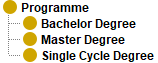
\includegraphics[width=.7\linewidth]{img/classes-programme-hierarchy.png}
         \caption{Gerarchia delle classi sui corsi di laurea.}\label{figs:programme-hierarchy}
       \end{minipage}\hfill
       \begin{minipage}{0.48\textwidth}
         \centering
         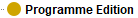
\includegraphics[width=.7\linewidth]{img/classes-programme-edition.png}
         \caption{Edizione del Corso di Laurea.}\label{figs:programme-edition}
       \end{minipage}
    \end{figure}
    
    \item \textbf{Course} - Classe usata per descrivere gli insegnamenti presenti in un corso di laurea, come con "Programme" si è gestito il problema degli insegnamenti e delle loro edizioni negli anni, infatti i corsi possono modificarsi, cambiare dei libri di testo, professori che li insegnano ma continuare ad avere proprietà in comune, ad esempio nell'università di Bologna i corsi presentano dei codici che rimangono i medesimi per piccoli cambiamenti del corso. Tali informazioni possono essere utili anche quando si confrontano insegnamenti di università diverse e vedere quali esami già sostenuti da uno studente potrebbero non essere risostenuti cambiando università o corso di laurea;
    
    \item \textbf{Department} - Classe per descrivere i dipartimenti di un'università. Essi costituiscono la struttura organizzativa della ricerca scientifica e delle attività didattiche e formative; fanno riferimento direttamente all'università (abbiamo constatato che i dipartimenti di UniBo non sono relativi ai campus ma all'università stessa);

    \item \textbf{Settore Scientifico Disciplinare} - [\textcolor{red}{VALUTARE se usare la classe ScientificDisciplinarySector di Ontopia https://w3id.org/italia/controlled-vocabulary/classifications-for-universities/academic-disciplines/}]

    \item \textbf{Event} - Classe utilizzata per descrivere eventi universitari di varia natura, nell'implementazione presentata vengono modellati \textbf{Exam} e \textbf{Lesson} come sotto classi di una classe intermedia fra loro ed Event: \textbf{Didactic Event}, che rappresenta gli eventi didattici universitari.
    \centeredImage{img/classes-event-hierarchy.png}{Gerarchia delle classi sugli eventi universitari}{0.30}{\label{figs:event-hierarchy}}
    
\end{itemize}

\section{Proprietà oggetto}

Le proprietà oggetto nell'ontologia vanno a mostrare una sottile gerarchia delle diverse classi, questo perché, ad esempio, un campus fa parte di un'università, un corso di laurea fa riferimento ad un campus, un insegnamento ad un CdL, ecc.

Nella maggior parte dei casi le diverse proprietà oggetto presentano anche la proprietà inversa perché strettamente correlati. Prendendo ad esempio il caso della relazione "ha campus" per le università, è presente anche la relazione inversa "è campus di".

Le proprietà che presentano la relazione inversa sono:

\begin{itemize}
    
    \objPropertyInv{has department}{is department of}{Organization}{Department}%
    {Proprietà che permette di legare dei dipartimenti ad un'università. \textcolor{red}{VALUTARE SE AGGIUNGERE ALTRO}}
  
    \objPropertyInv{has campus}{is campus of}{Organization}{Campus}%
    {Proprietà utilizzata per indicare i campus relativi ad un'università, la proprietà inversa permette di risalire all'università di cui fa parte il campus della relazione.
    \\
    Così come nella realtà, un'università può avere più campus.}

    \objPropertyInv{has programme}{is programme of}{Campus}{Programme}%
    {Proprietà che mette in relazione un campus e un Corso di Laurea da esso fornito; un campus può avere più CdL inoltre il legame che intercorre fra i due non implica che le lezioni degli insegnamenti di un corso di laurea avvengano nel campus di cui quest'ultimo è parte.}

    \objPropertyInv{has programme edition}{is programme edition of}{Programme}{Programme Edition}%
    {Proprietà che permette di denotare l'edizione di un Corso di Laurea, questo per permettere di avere ogni anno dei cambiamenti come spesso avviene, in questo modo possono cambiare i corsi che lo compongono e modificare anche l'ordine degli esami negli anni e/o semestri.}

    \objPropertyInv{has programme year}{is programme year of}{Programme Edition}{Programme Year}%
    {Proprietà per creare la relazione l'edizione di un Corso di Laurea con gli anni da cui esso è composto. Le triennali avranno quindi primo, secondo e terzo anno, le magistrali primo e secondo (relativamente al tipo di magistrale), ecc.}
    
    \objPropertyInv{has course}{is course of}{Programme Year}{Course Edition}{\textcolor{red}{se usassimo has course edition al posto di questa?}}

    \objPropertyInv{has course edition}{is course edition of}{Course}{Course Edition}%
    {Proprietà che permette di avere differenti edizioni di un insegnamento, così come avviene per i corsi di laurea. In diverse università i corsi mantengono le stesse informazioni principali, come codici che li distinguono, ma effettuano dei cambiamenti negli anni come ad esempio fare riferimento a differenti libri di testo, cambiare le modalità di esame, cambiare semestre, ecc. Questa modellazione permette di farlo andando a creare un nuovo corso ogni anno.
    \textcolor{red}{e se questa proprietà la usassimo anche per gli anni? così da non creare un'ulteriore proprietà usabile con una sola classe.}}

    \objPropertyInv{has exam}{is exam of}{Course Edition}{Exam}%
    {Proprietà usata per indicare gli esami di un insegnamento.}
    
    \objPropertyInv{has lecture}{is lecture of}{Course Edition}{Lecture}%
    {Proprietà usata per indicare le lezioni di un insegnamento.}

    \objPropertyInv{has room}{is room of}{Campus}{Room}%
    {Proprietà usata per indicare le stanze presenti in un campus, esse possono essere di varia natura come si è visto in \cref{figs:location-hierarchy}/}

    \objPropertyInv{teaches}{is taught by}{Professor}{Course Edition}%
    {Proprietà usata per descrivere la relazione fra un professare e gli insegnamenti da lui tenuti. Siccome la relazione ha come dominio le edizioni dei corsi, ogni anno un professore è legato nuovamente con il medesimo corso se continua ad insegnarlo. Lo abbiamo però ritenuto opportuno dato che ciò permette di tenere traccia degli insegnamenti tenuti nei diversi anni da un professore.}

\end{itemize}

Le proprietà che oggetto che non presentano una relazione inversa sono di un numero abbastanza inferiore rispetto le precedenti e abbiamo:

\begin{itemize}
  \objPropertyNotInv{belongs to department}{Professor}{Department}%
  {Proprietà che permette di descrivere la relazione fra un professore e il dipartimento di cui fa parte.}

  \objPropertyNotInv{belongs to scientific disciplinary area}{Professor, Course}{Scientific Disciplinary Area}%
  {Proprietà che permette di modellare la relazione di appartenza ad un settore scientifico disciplinare (SSD). Tale proprietà è presente sia per i professori sia per gli insegnamenti erogati. Osservando le strutture organizzative delle università abbiamo constato che tale appartenenza vincola i professori ad insegnare corsi del medesimo SSD a cui essi appartengono, quindi un professore di un SSD può insegnare un corso con SSD differente.}

  \objPropertyNotInv{has course book}{Course Edition}{Book}
  {Proprietà usata per descrivere la relazione fra l'edizione di un insegnamento e i libri di testo che vengono utilizzati. "Book" è una classe dell'ontologia Bibo importata all'interno del progetto.}
\end{itemize}

\section{Proprietà dei dati}

\textcolor{red}{AGGIUNGERE NELL'ONTOLOGIA E NELLA RELAZIONE}